% Options for packages loaded elsewhere
\PassOptionsToPackage{unicode}{hyperref}
\PassOptionsToPackage{hyphens}{url}
%
\documentclass[
  man,floatsintext]{apa7}
\usepackage{amsmath,amssymb}
\usepackage{iftex}
\ifPDFTeX
  \usepackage[T1]{fontenc}
  \usepackage[utf8]{inputenc}
  \usepackage{textcomp} % provide euro and other symbols
\else % if luatex or xetex
  \usepackage{unicode-math} % this also loads fontspec
  \defaultfontfeatures{Scale=MatchLowercase}
  \defaultfontfeatures[\rmfamily]{Ligatures=TeX,Scale=1}
\fi
\usepackage{lmodern}
\ifPDFTeX\else
  % xetex/luatex font selection
\fi
% Use upquote if available, for straight quotes in verbatim environments
\IfFileExists{upquote.sty}{\usepackage{upquote}}{}
\IfFileExists{microtype.sty}{% use microtype if available
  \usepackage[]{microtype}
  \UseMicrotypeSet[protrusion]{basicmath} % disable protrusion for tt fonts
}{}
\makeatletter
\@ifundefined{KOMAClassName}{% if non-KOMA class
  \IfFileExists{parskip.sty}{%
    \usepackage{parskip}
  }{% else
    \setlength{\parindent}{0pt}
    \setlength{\parskip}{6pt plus 2pt minus 1pt}}
}{% if KOMA class
  \KOMAoptions{parskip=half}}
\makeatother
\usepackage{xcolor}
\usepackage{graphicx}
\makeatletter
\def\maxwidth{\ifdim\Gin@nat@width>\linewidth\linewidth\else\Gin@nat@width\fi}
\def\maxheight{\ifdim\Gin@nat@height>\textheight\textheight\else\Gin@nat@height\fi}
\makeatother
% Scale images if necessary, so that they will not overflow the page
% margins by default, and it is still possible to overwrite the defaults
% using explicit options in \includegraphics[width, height, ...]{}
\setkeys{Gin}{width=\maxwidth,height=\maxheight,keepaspectratio}
% Set default figure placement to htbp
\makeatletter
\def\fps@figure{htbp}
\makeatother
\setlength{\emergencystretch}{3em} % prevent overfull lines
\providecommand{\tightlist}{%
  \setlength{\itemsep}{0pt}\setlength{\parskip}{0pt}}
\setcounter{secnumdepth}{-\maxdimen} % remove section numbering
% Make \paragraph and \subparagraph free-standing
\ifx\paragraph\undefined\else
  \let\oldparagraph\paragraph
  \renewcommand{\paragraph}[1]{\oldparagraph{#1}\mbox{}}
\fi
\ifx\subparagraph\undefined\else
  \let\oldsubparagraph\subparagraph
  \renewcommand{\subparagraph}[1]{\oldsubparagraph{#1}\mbox{}}
\fi
\ifLuaTeX
\usepackage[bidi=basic]{babel}
\else
\usepackage[bidi=default]{babel}
\fi
\babelprovide[main,import]{american}
% get rid of language-specific shorthands (see #6817):
\let\LanguageShortHands\languageshorthands
\def\languageshorthands#1{}
% Manuscript styling
\usepackage{upgreek}
\captionsetup{font=singlespacing,justification=justified}

% Table formatting
\usepackage{longtable}
\usepackage{lscape}
% \usepackage[counterclockwise]{rotating}   % Landscape page setup for large tables
\usepackage{multirow}		% Table styling
\usepackage{tabularx}		% Control Column width
\usepackage[flushleft]{threeparttable}	% Allows for three part tables with a specified notes section
\usepackage{threeparttablex}            % Lets threeparttable work with longtable

% Create new environments so endfloat can handle them
% \newenvironment{ltable}
%   {\begin{landscape}\centering\begin{threeparttable}}
%   {\end{threeparttable}\end{landscape}}
\newenvironment{lltable}{\begin{landscape}\centering\begin{ThreePartTable}}{\end{ThreePartTable}\end{landscape}}

% Enables adjusting longtable caption width to table width
% Solution found at http://golatex.de/longtable-mit-caption-so-breit-wie-die-tabelle-t15767.html
\makeatletter
\newcommand\LastLTentrywidth{1em}
\newlength\longtablewidth
\setlength{\longtablewidth}{1in}
\newcommand{\getlongtablewidth}{\begingroup \ifcsname LT@\roman{LT@tables}\endcsname \global\longtablewidth=0pt \renewcommand{\LT@entry}[2]{\global\advance\longtablewidth by ##2\relax\gdef\LastLTentrywidth{##2}}\@nameuse{LT@\roman{LT@tables}} \fi \endgroup}

% \setlength{\parindent}{0.5in}
% \setlength{\parskip}{0pt plus 0pt minus 0pt}

% Overwrite redefinition of paragraph and subparagraph by the default LaTeX template
% See https://github.com/crsh/papaja/issues/292
\makeatletter
\renewcommand{\paragraph}{\@startsection{paragraph}{4}{\parindent}%
  {0\baselineskip \@plus 0.2ex \@minus 0.2ex}%
  {-1em}%
  {\normalfont\normalsize\bfseries\itshape\typesectitle}}

\renewcommand{\subparagraph}[1]{\@startsection{subparagraph}{5}{1em}%
  {0\baselineskip \@plus 0.2ex \@minus 0.2ex}%
  {-\z@\relax}%
  {\normalfont\normalsize\itshape\hspace{\parindent}{#1}\textit{\addperi}}{\relax}}
\makeatother

\makeatletter
\usepackage{etoolbox}
\patchcmd{\maketitle}
  {\section{\normalfont\normalsize\abstractname}}
  {\section*{\normalfont\normalsize\abstractname}}
  {}{\typeout{Failed to patch abstract.}}
\patchcmd{\maketitle}
  {\section{\protect\normalfont{\@title}}}
  {\section*{\protect\normalfont{\@title}}}
  {}{\typeout{Failed to patch title.}}
\makeatother

\usepackage{xpatch}
\makeatletter
\xapptocmd\appendix
  {\xapptocmd\section
    {\addcontentsline{toc}{section}{\appendixname\ifoneappendix\else~\theappendix\fi\\: #1}}
    {}{\InnerPatchFailed}%
  }
{}{\PatchFailed}
\keywords{keywords\newline\indent Word count: TBC}
\usepackage{csquotes}
\raggedbottom
\ifLuaTeX
  \usepackage{selnolig}  % disable illegal ligatures
\fi
\IfFileExists{bookmark.sty}{\usepackage{bookmark}}{\usepackage{hyperref}}
\IfFileExists{xurl.sty}{\usepackage{xurl}}{} % add URL line breaks if available
\urlstyle{same}
\hypersetup{
  pdftitle={Study 3},
  pdfauthor={Blinded1, Blinded2, Blinded1, \& Blinded1},
  pdflang={en-US},
  pdfkeywords={keywords},
  hidelinks,
  pdfcreator={LaTeX via pandoc}}

\title{Study 3}
\author{Blinded\textsuperscript{1}, Blinded\textsuperscript{2}, Blinded\textsuperscript{1}, \& Blinded\textsuperscript{1}}
\date{}


\shorttitle{Moral Dilution}

\authornote{

Correspondence concerning this article should be addressed to Blinded, Blinded. E-mail: Blinded

}

\affiliation{\vspace{0.5cm}\textsuperscript{1} Blinded\\\textsuperscript{2} Blinded}

\abstract{%
Six studies etc.
}



\begin{document}
\maketitle

\hypertarget{study-3---good-and-bad-characters}{%
\section{Study 3 - Good and Bad Characters}\label{study-3---good-and-bad-characters}}

In Study 1 we found evidence for the moral dilution effect for judgments of \emph{bad} moral characters. In Study 2 we failed replicate this effect for judgments of \emph{good} moral characters. The aim of Study 3 was to test if valence (good vs.~bad) moderates the moral dilution effect. We hypothesized that valence (good vs bad) would interact with condition in producing a dilution effect, such that the dilution effect would be observed for bad characters but not for good characters. Study 3 was pre-registered at \color{blue}\url{https://aspredicted.org/QDF_XT1}\color{black}.

\hypertarget{study-3-method}{%
\subsection{Study 3: Method}\label{study-3-method}}

\hypertarget{study-3-participants-and-design}{%
\subsubsection{Study 3: Participants and design}\label{study-3-participants-and-design}}

Study 3 was a 2 \(\times\) 2 within-subjects factorial design. The first independent variable was condition with two levels, diagnostic and non-diagnostic. The second independent variable was valence of character description, with two levels morally good and morally bad. We used the same two dependent variables as in previous studies, the four item moral perception scale (MPS-4, \(\alpha\) = 0.97), and the single item moral perception measure MM-1.

A total sample of 1386 (758 female, 535 male, 10 non-binary, 2 other; 11 prefer not to say, \emph{M}\textsubscript{age} = 29.67, min = 0.36, max = 70, \emph{SD} = 8.97) started the survey. Participants were recruited from MTurk and paid \$0.40 for their participation.

Participants who failed both manipulation checks were removed (\emph{n} = 541), leaving a total sample of 828.75 participants (327 female, 462 male, 2 other, 2 prefer not to say; \emph{M}\textsubscript{age} = 26.03, min = 11, max = 70, \emph{SD} = 9.53).

\hypertarget{study-3-procedure-and-materials}{%
\subsubsection{Study 3: Procedure and materials}\label{study-3-procedure-and-materials}}

Again, data were collected using an online questionnaire presented with Qualtrics (www.qualtrics.com). Participants were presented with four descriptions of characters taken from Studies 1 and 2. To ensure consistency across character judgments, we selected descriptions that related to the same moral foundations (care, fairness, and loyalty). We used the same four character names as in previous studies. The \emph{good} characters were \emph{Sam} and \emph{Robin}, and the \emph{bad} characters were \emph{Francis} and \emph{Alex}, e.g., \emph{Imagine a person named Robin. Throughout their life they have been known to show compassion and empathy for others, act with a sense of fairness and justice, and, never to break their word.} or, \emph{Imagine a person named Alex. Throughout their life they have been known to be cruel, act unfairly, and to betray their own group.} Full descriptions for each character are in the supplementary materials. One description for each the \emph{good} and \emph{bad} characters was randomly assigned to include non-diagnostic information for each participant thus all participants were exposed to all conditions (see \color{blue}\url{https://osf.io/mdnpv/?view_only=77883e3fbc3d45f1a35fe92d5318cb67}\color{black} for details of the randomization blocks). Study 3 was pre-registered at \color{blue}\url{https://aspredicted.org/QDF_XT1}\color{black}

\hypertarget{study-3-results}{%
\subsection{Study 3: Results}\label{study-3-results}}

The means and standard deviations for MPS-4 for each scenario are as follows:
\emph{Sam} (good),
\emph{M}\textsubscript{MPS-4} = 6.20, \emph{SD}\textsubscript{MPS-4} = 0.81,
\emph{Francis} (bad),
\emph{M}\textsubscript{MPS-4} = 2.15, \emph{SD}\textsubscript{MPS-4} = 0.79,
\emph{Alex} (bad),
\emph{M}\textsubscript{MPS-4} = 2.32, \emph{SD}\textsubscript{MPS-4} = 0.89,
\emph{Robin} (good),
\emph{M}\textsubscript{MPS-4} = 6.32, \emph{SD}\textsubscript{MPS-4} = 0.76. There was significant variation depending on the description, \emph{F}(2,1515) = 6,251.52, \emph{p} \textless{} .001, partial \(\eta\)\textsuperscript{2} = 0.86. Both the \emph{good} characters (\emph{Robin} and \emph{Sam}) were rated significantly more favorably than both the \emph{bad} characters (\emph{Alex} and \emph{Francis}; all \emph{p}s \textless{} .001). There were no differences between \emph{Robin} and \emph{Sam} (\emph{good}: \emph{p} = .003) or between \emph{Alex} and \emph{Francis} (\emph{bad}; \emph{p} \textless{} .001).

The means and standard deviations for MM-1 for each scenario are as follows:
\emph{Sam} (good),
\emph{M}\textsubscript{MM-1} = 86.33, \emph{SD}\textsubscript{MM-1} = 13.68;
\emph{Francis} (bad),
\emph{M}\textsubscript{MM-1} = 20.25, \emph{SD}\textsubscript{MM-1} = 16.93;
\emph{Alex} (bad),
\emph{M}\textsubscript{MM-1} = 23.07, \emph{SD}\textsubscript{MM-1} = 17.51;
\emph{Robin} (good),
\emph{M}\textsubscript{MM-1} = 88.44, \emph{SD}\textsubscript{MM-1} = 12.00. There was significant variation depending on the description, \emph{F}(2,1380) = 5,282.47, \emph{p} \textless{} .001, partial \(\eta\)\textsuperscript{2} = 0.826. Again, the \emph{good} characters (\emph{Robin} and \emph{Sam}) were rated significantly more favorably than the \emph{bad} characters (\emph{Alex} and \emph{Francis}; all \emph{p}s \textless{} .001). There were no differences between \emph{Robin} and \emph{Sam} (\emph{good}: \emph{p} = .001) or between \emph{Alex} and \emph{Francis} (\emph{bad}; \emph{p} \textless{} .001).

We conducted a linear-mixed-effects model to test if our predictors influenced MPS-4 responses. Our outcome measure was MPS-4, our predictor variables were condition and valence; we allowed intercepts and the effects of condition and valence to vary across participants.
Overall, the model significantly predicted participants responses, and provided a better fit for the data than the baseline model,
\(\chi\)\textsuperscript{2}(5) = 2,733.13, \emph{p} \textless{} .001.
Overall, there was a significant main effect for condition,
\emph{F}(1, 825) = 47.54, \emph{p} \textless{} .001;
valence significantly predicted responses,
\emph{F}(1, 823) = 3,423.33, \emph{p} \textless{} .001;
and there was a significant condition \(\times\) valence interaction,
\emph{F}(1, 819) = 6.56, \emph{p} = .011.

We conducted a linear-mixed-effects model to test if our predictors influenced MM-1 responses. The model was the same as the previous model, with a change to the outcome measure, our outcome measure for this model was MM-1. As above, our predictor variables were condition and valence; we allowed intercepts and the effects of condition and valence to vary across participants.
Overall, the model significantly predicted participants responses, and provided a better fit for the data than the baseline model,
\(\chi\)\textsuperscript{2}(5) = 6,652.62, \emph{p} \textless{} .001.
Overall there was a main effect for condition,
\emph{F}(1, 829) = 30.29, \emph{p} \textless{} .001;
valence significantly predicted responses,
\emph{F}(1, 824) = 273.59, \emph{p} \textless{} .001;
and there was no significant condition \(\times\) valence interaction,
\emph{F}(1, 825) = 1.57, \emph{p} = .211.

For both MP-4 and MM-1 we found a main effect for condition and valence, and there was a condition \(\times\) valence interaction for MP-4 but not for MM-1. We conducted follow-up analyses to test the if the main effect for condition holds for both good and bad descriptions separately.

\hypertarget{differences-in-the-bad-descriptions}{%
\subsection{\texorpdfstring{Differences in the \emph{Bad} Descriptions}{Differences in the Bad Descriptions}}\label{differences-in-the-bad-descriptions}}

We conducted a linear-mixed-effects model to test if condition influenced MPS-4 responses. Our outcome measure was MPS-4, our predictor variable was condition; we allowed intercepts and the effect of condition to vary across participants. Overall, the model significantly predicted participants responses, and provided a better fit for the data than the baseline model, \(\chi\)\textsuperscript{2}(3) = 77.91, \emph{p} \textless{} .001. Condition significantly influenced MPS-4 responses \emph{F}(1, 818.61) = 46.18, \emph{p} \textless{} .001, and was a significant predictor in the model \(b\) = -0.10, \emph{t}(818.61) = -6.80, \emph{p} \textless{} .001, see Figure~\ref{fig:S3bothconditionplot}.

We conducted a linear-mixed-effects model to test if condition influenced MM-1 responses. Our outcome measure was MM-1, our predictor variable was condition; we allowed intercepts and the effect of condition to vary across participants. Overall, the model significantly predicted participants responses, and provided a better fit for the data than the baseline model, \(\chi\)\textsuperscript{2}(3) = 47.56, \emph{p} \textless{} .001. Condition significantly influenced MM-1 responses \emph{F}(1, 822.47) = 19.21, \emph{p} \textless{} .001, and was a significant predictor in the model \(b\) = -1.13, \emph{t}(822.47) = -4.38, \emph{p} \textless{} .001, see Figure~\ref{fig:S3bothconditionplot}.

\hypertarget{differences-in-the-good-descriptions}{%
\subsection{\texorpdfstring{Differences in the \emph{Good} Descriptions}{Differences in the Good Descriptions}}\label{differences-in-the-good-descriptions}}

We conducted a linear-mixed-effects model to test if condition influenced MPS-4 responses. Our outcome measure was MPS-4, our predictor variable was condition; we allowed intercepts and the effect of condition to vary across participants. Overall, the model significantly predicted participants responses, and provided a better fit for the data than the baseline model, \(\chi\)\textsuperscript{2}(3) = 31.37, \emph{p} \textless{} .001. Condition significantly influenced MPS-4 responses \emph{F}(1, 826.37) = 11.61, \emph{p} \textless{} .001, and was a significant predictor in the model \(b\) = 0.05, \emph{t}(826.37) = 3.41, \emph{p} \textless{} .001, see Figure~\ref{fig:S3bothconditionplot}.

\begin{figure}
\centering
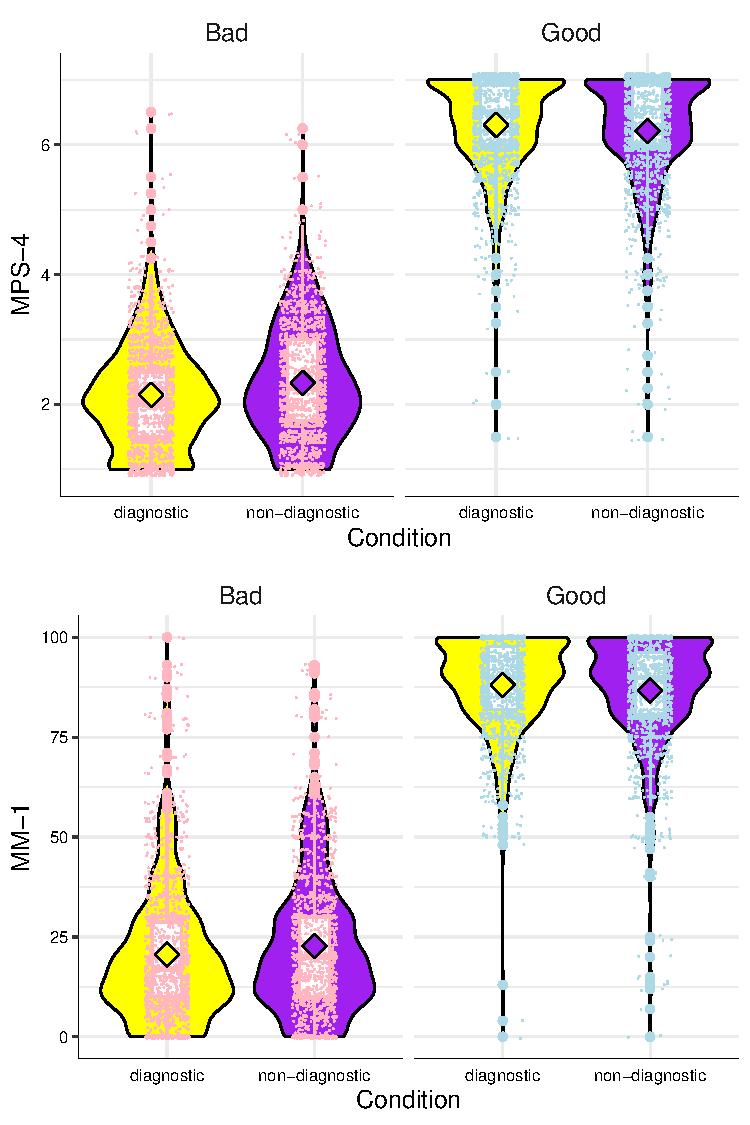
\includegraphics{Study_6_files/figure-latex/S3bothconditionplot-1.pdf}
\caption{\label{fig:S3bothconditionplot}Study 3: Differences in moral perception depending on condition}
\end{figure}

We conducted a linear-mixed-effects model to test if condition influenced MM-1 responses. Our outcome measure was MM-1, our predictor variable was condition; we allowed intercepts and the effect of condition to vary across participants. Overall, the model significantly predicted participants responses, and provided a better fit for the data than the baseline model, \(\chi\)\textsuperscript{2}(3) = 43.43, \emph{p} \textless{} .001. Condition significantly influenced MM-1 responses \emph{F}(1, 825) = 13.96, \emph{p} \textless{} .001, and was a significant predictor in the model \(b\) = 0.71, \emph{t}(825) = 3.74, \emph{p} \textless{} .001, see Figure~\ref{fig:S3bothconditionplot}.


\end{document}
